\chapter{Results}\label{chapter:results}
Following providing the multivariate analysis technique described in Section~\ref{sec:mvas} with the simulated samples, and their systematic variations, and data, the resultant set of BDT discriminator distributions can be used to perform a measurement.

The following chapter describes the statistical methodology used to analyses these distributions and produce the blinded measurement of the upper limit of the signal process' cross section along with its expected significance.
Following a discussion of the impact that the systematic uncertainties have on the fitted results, the blinded result presented is compared with that from the already published trileptonic final state for tZq production.

\section{Statistical Methodology}\label{sec:statisticalModel}
The Higgs Analysis Combined Limit (\combine) tool~\cite{Combine} tool, a framework based on the RooStats package~\cite{Moneta:2010pm,Schott:2012zb}, was used to perform a binned Maximum Likelihood Fit (MLF) to analyses the measurement made using the $CL_{S}$ method~\cite{CMS-NOTE-2011-005,Khachatryan:2014jba,AsymptoticFormulae}.

\subsection{Likelihood Model}\label{subsec:likelihoodModel}
For the signal and background processes considered in the search, the expected event yield $\lambda$ in bin $i$ of the distribution considered (\ie the BDT discriminator) is given by Equation~(\ref{eq:yields1}):

\begin{equation}
\lambda_{i} = \mu s_{i} + \sum\limits_{j}^{n_{bkgs}} b_{j} \;
\label{eq:yields1}
\end{equation}

where $s$ and $b$ are the expected number of signa, and background events, respectively, the index $j$ runs over the number of background sources, $n_{bkgs}$, and $\mu$ is the signal strength modifier.
The signal strength modifier is typically used instead of directly determining the expected (and observed) cross section of a process as it makes the comparison of different results (particularly from different experiments) more straightforward. 
The relationship between $\mu$ and the observed and expected cross sections, $\sigma_{obs}$ and $\sigma_{s}$, is given by Equation(~\ref{eq:signalModifier}):

\begin{equation}
\mu = \frac{\sigma_{obs}}{\sigma_{s}}  \;
\label{eq:signalModifier}
\end{equation}
 
The uncertainties associated with the simulated predictions for the signal and background processes are accounted for by the inclusion of a set of nuisance parameters $\theta$.
Therefore, as $s_{i}$ and $b_{i}$ are dependent on $\theta$, they become $s_{i} = s_{i} (\theta)$ and $b_{i} = b_{i} (\theta)$.

Assuming that the number of observed events, $n_{i}$, in any given bin of the distribution considered will be distributed according to Poisson statistics, the probability of observing $n_{i}$ is given by Equation~(\ref{eq:poissonProb}):

\begin{equation}
\mathcal{P} ( n_{i} | \lambda_{i} ) = \frac{\lambda_{i}}{n_{i}!} e^{- \lambda_{i}} = \frac{ \big( \mu s_{i}(\theta) + b_{i}(\theta) \big)^{n_{i}}}{n_{i} !} e^{- \mu s_{i}(\theta) - b_{i}(\theta)}  \;
\label{eq:poissonProb}
\end{equation}

A probability density function, $\rho ( \theta | \tilde{\theta} )$ is used to describe all the sources of uncertainty for the nuisance parameters, where $\tilde{\theta}$ is the set of nominal values for the the best estimate of the nuisances.
For the search presented in this thesis, it is assumed that each source of systematic uncertainty is either 100\% correlated or uncorrelated.
This allows each systematic uncertainty to be incorporated into the likelihood function in a clean factorised form.
Shape uncertainties are modelled by vertically morphing the nominal shape template up and down by one $\sigma$.
The non-prompt lepton normalisation and luminosity flat rate uncertainties are treated as log-uniform and log-normal distributed nuisance parameters respectively~\cite{Baak:2014fta,AsymptoticFormulae}.
%%% log-uniform - for NPL to allow it to be simultaneously fitted with the signal normalisation

Thus, the likelihood for the entire dataset can be expressed as the product of the Poisson probabilities, $\mathcal{P}$, for all bins and the nuisance parameters' probability density function, as given by Equation~(\ref{eq:poissonLikelihood}).

\begin{equation}
\mathcal{L} ( n_{i} | \mu , \theta ) = 
\prod_{i=1}^{N} \mathcal{P} \big( n_{i} | \mu s_{i}(\theta) + b_{i}(\theta) \big) \rho ( \theta | \tilde{\theta} ) \;
\label{eq:poissonLikelihood}
\end{equation}

\subsection{$CL_{S}$ method}\label{subsec:CLsMethod}
The modified classical frequentist method, known as the $CL_{S}$ method, was used to evaluate the compatibility of data with the \emph{signal plus background} (s+b) and \emph{background only} (b-only) hypotheses in terms of the signifiance of, and the limits on, the measured signal strength ~\cite{AsymptoticFormulae}.

To evaluate these hypotheses, the $CL_{S}$ method constructs a test statistic, $q_{\mu}$.
The test statistic used by the ATLAS and CMS is defined as the loglikelihood ratio in equation~\ref{eq:testStatistic},

\begin{equation}
q_{\mu} =  -2 \ln \frac{ \mathcal{L}(data | \mu s , \hat{\theta_{\mu}})} { \mathcal{L}(data | \hat{\mu} s \hat{\theta_{\mu})  }} \textrm{ , where } 0 \leq \hat{\mu} \leq \mu \;
\label{eq:testStatistic}
\end{equation}

where $\hat{\theta_{\mu}}$ refers to the maximum likelihood estimators of $\theta$ for a given $\mu$, and 
$\hat{\mu}$ and $\hat{\theta}$ correspond to the global maximum of the likelihood. 
By definition $\hat{\mu}$ cannot take negative values as physics defines the signal rate as positive. 
The constraint $\hat{\mu} < \mu$ is applied to ensure a one-sided confidence interval.

As the analysis is initially conducted blind, \emph{pseudodata} is generated using toy MC for the \emph{expected} outcomes in order to construct probability distribution functions for the s+b and b-only hypotheses for a given signal strength.
For the unblinding of the analysis, the \emph{observed} measurement will be made by replacing the pseudodata used for the s+b probability distribution functions with the actual data.
From these probability distribution functions, the probability values for the s+b and b-only hypotheses can be defined as Equations~(\ref{eq:pmu})-(~\ref{eq:1-pb}):

\begin{equation}
p_{\mu} = P ( q_{\mu} \geq  q_{\mu}^{obs} | \mu s + b ) = \int^{\infty}_{q_{\mu}^{obs}} f ( q_{\mu} | \mu , \theta_{\mu}^{obs} ) dq_{\mu} \;
\label{eq:pmu}
\end{equation}

\begin{equation}
1 - p_{b} = P ( q_{\mu} \geq  q_{\mu}^{obs} | b ) = \int^{\infty}_{q_{0}^{obs}} f ( q_{\mu} | 0 , \theta_{0}^{obs} ) dq_{\mu} \;
\label{eq:1-pb}
\end{equation}

The ratio of these probabilities is used to define $CL_{S} (\mu)$ in Equation~(\ref{eq:CLs}).

\begin{equation}
CL_{S} (\mu) = \frac{ p_{\mu} }{ 1 - p_{b} }\;
\label{eq:CLs}
\end{equation}

If, for a given $\mu$, $CL_{S} < \alpha$, then it is said that the signal process in question is excluded with a $(1 - \alpha)$ Confidence Level (CL).
Therefore, as the 95\% CL upper limit is used in this search, the limit is determined by altering $\mu$  until $CL_{S} = 0.05$.

%\subsection{Asymptotic CL$_{s}$ method}\label{subsec:asymptoticCLS}
Instead of using an ensemble of toy MC samples to generate the pseudodata, one representative dataset, known as the \emph{Asimov dataset}, was used.
This method, known as the \emph{asymptotic} CL$_{s}$ method, is used when the number of expected events is sufficiently large as it typically reduces the amount of computing time required.
The Asimov dataset is defined as being constructed such that all observable quantities are equal to their expectation values.
A full description of the asymptotic approximation to the CL$_{s}$ method is given in~\cite{AsymptoticFormulae}.

\section{Statistical Analysis Results}\label{sec:results}
For the combination of both final states, at 95\% CL, the expected signal strength for tZq production was determined to be $1.0^{+1.011}_{-1.045}$, corresponding to an expected significance of $0.95 \sigma$.
Using the reference NLO cross section of $\sigma (tZq, Z \rightarrow l^{+} l^{-}$) = 94.2 fb~\cite{Campbell:2013yla}, given in Section~\ref{}, this results corresponds to an expected cross section of $94.2^{+95.3}_{-98.4475}$.
This is both consistent with the SM prediction and the cross sections of measurements of $70.65 \pm 25.9$ and $137^{+45}_{-40}$ that were made by the ATLAS and CMS collaborations, respectively, using the trilepton final state at $\sqrt{s} = 13 \TeV$~\cite{Aaboud:2017ylb,Sirunyan:2017nbr}.

The blinded expected signal strengths, expected cross sections, and expected significances for the individual channels and their combination are shown in full in Table~\ref{tab:shapetxs}.

\begin{table}[!h]
   \centering
   \caption{The expected signal strengths and corresponding cross sections for
   the individual channels and the channels combined at the 95\% CL.}
   \begin{tabular}{cccc}
       \hline
       Channel & $ee$ & $\mu\mu$ & \textbf{Combination} \\
        \hline
       Cross section (fb) & $X_{-Z}^{+Y}$ & $X_{-Z}^{+Y}$ & $X_{-Z}^{+Y}$ \\
       Significance (expected) ($\sigma$) & $0.644448_{-Z}^{+Y}$ & $1.63987_{-Z}^{+Y}$ & $1.77376_{-Z}^{+Y}$ \\
%       Significance (observed) ($\sigma$) & $X_{-Z}^{+Y}$ & $X_{-Z}^{+Y}$ & $X_{-Z}^{+Y}$ \\
    \end{tabular}
   \label{tab:shapetxs}
\end{table}

In order to improve on this result, this analysis is being extended to incorporate 2017 in accordance with CMS policy.

\section{Post-Fit Impact of the Systematic Uncertainties}\label{sec:uncertainitiesImpact}
The impact of each of the sources of systematic uncertainty on the signal strength modifier $\mu$ is shown shown in Figure~\ref{fig:systematicsPull}, where the left hand side of the plot illustrates the nuisance parameter residuals and the right hand side the impact of varying a nuisance parameter to its $\pm \sigma$ post-fit values has on the $\mu$.

%Given the background dominated nature of this search, it is not too surprising that the uncertainty on the luminosity %has the single largest impact on $\mu$.
%As Figure~\ref{fig:systematicsPull} shows, while the maximum likelihood fit does constrain the impact of this uncertainty on the 
%

%Requiring variables constructed from the multiple jets in the final state, such as $m_{top}$, increases the sensitivity of these parameters to the resolution of the HCAL.
%
%The impact of the other experimental uncertainties are either smaller than or of the same scale as the least impactful theoretical uncertainties.
%The uncertainties in the matching of the ME and PS 

%The theoretical uncertainties, while being well constrained during the 
%While the impact of the theoretical uncertainties were further constrained during the MLF, each source has a an impact on the measured signal strength equal to or greater than each of the experimental uncertainties do individually (except that of the luminosity measurement).
%
%As the  .... ISR+FSR+PS
%
%
%The uncertainties associated with the Jet Energy Resolutions and Parton Distribution 
%JER + PDF biggest experimental  
% 
%MET = small 
% 
%Despite the large conservative rate uncertainty ascribed to the non-prompt lepton fake shapes, 
%their
%
%given their relatively small contribution compared to other background processes and the effectiveness of the BDT in separating , the impact 

\begin{figure}[htbp]
\begin{center}
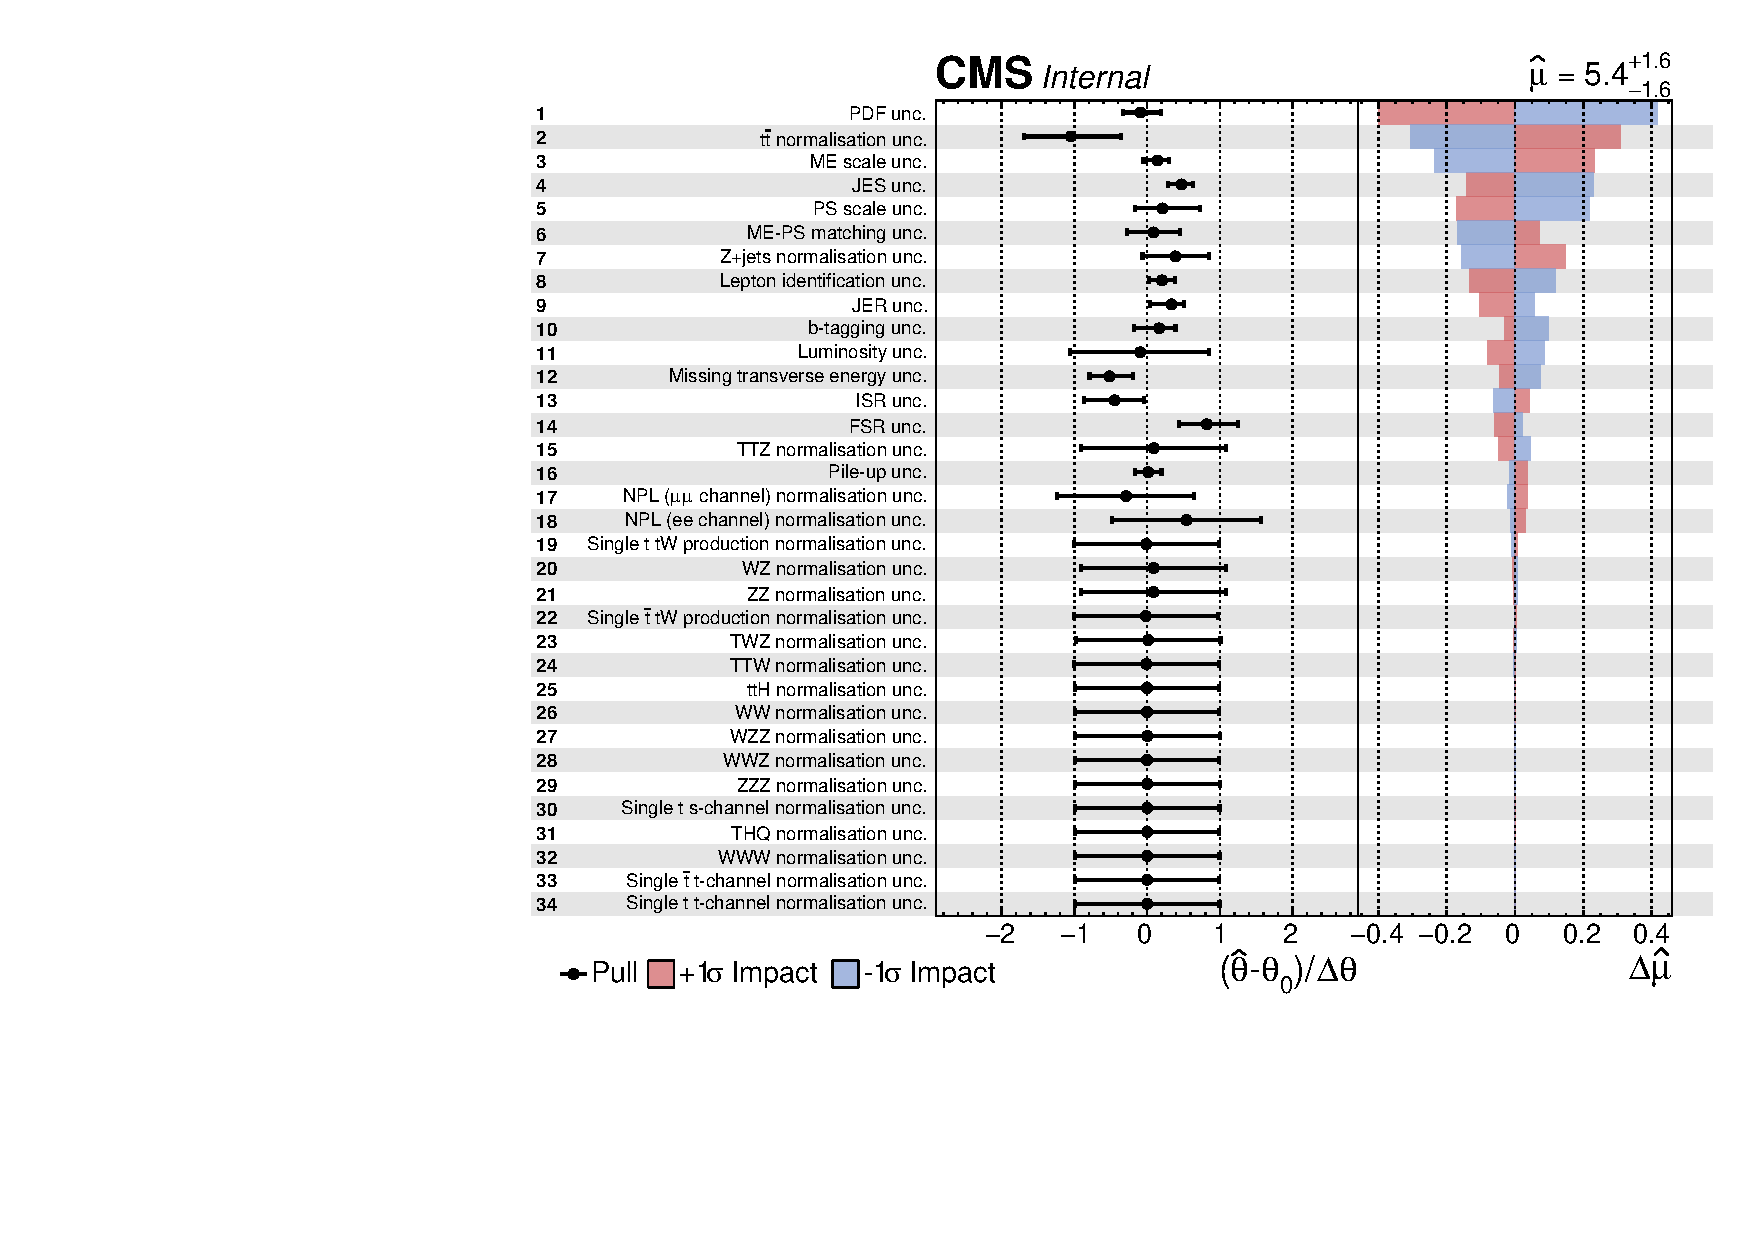
\includegraphics[width=0.97\textwidth]{figs/results/systematicsImpact.pdf}
\caption{The central values and uncertainties of the nuisance parameters (left-hand side) and the impact of each systematic uncertainty (when varied by $\pm 1 \sigma$) on the signal strength parameter $r$ following the fit
}
\label{fig:systematicsPull}
\end{center}
\end{figure}

\section{Discussion of other searches for tZq at the Large Hadron Collider}
The search for the decay of a single top produced in association with a Z boson presented in this thesis is the first one for the dilepton final state that has been undertaken at the LHC.
Previous searches for tZq production have been using the trilepton final state by the CMS collaboration at $\sqrt{s} = 8 \TeV$~\cite{Sirunyan:2017kkr} and by the ATLAS and CMS collaborations at $\sqrt{s} = 13 \TeV$~\cite{Aaboud:2017ylb,Sirunyan:2017nbr}.

The observed significances of the measurements made using the trilepton din4.2 $\sigma$ and 3.7 $\sigma$ reported by the ATLAS and CMS collaborations, respectively, when using the trilepton final state are considerably larger than the expected significance of $0.95 \sigma$ for the expected dilepton final state measurement.
The reason why the expected result made using dilepton final state is significantly less significant that of measurements made using the trilepton final state is a consequence of the size of the backgrounds for the two final states.

While the search using the dilepton final state is less sensitive to 

Requiring a third lepton in the final state suppresses backgrounds with only two leptons trilepton final state, by defi

Therefore, given that the lack of sufficient statistics is the main factor limiting the significance of the expected result presented, it is essential to extend this search to include additional data collected by the CMS experiment if tZq is to be observed using the dilepton final state.